\section{1D-Prototyp}
In diesem Teil wird der erste Prototyp vorgestellt. Hierbei handelt es sich um eine einzelne Würfelseite, welche mit Hilfe einer Achse gelagert ist. Dadurch wird die Bewegung des Systems auf zwei rotatorische Freiheitsgrade beschränkt, nämlich die Rotation um die Achse und die Bewegung der Schwungmasse relativ zu der Würfelseite. Mit Hilfe dieses Entwurfes kann die Dynamik und Anforderungen an die Komponenten an einem vereinfachten Modell untersucht werden. Aus diesen Ergebnisse können dann Rückschlüsse auf den Entwurf des endgültigen Würfels gezogen werden.
\newline


\begin{figure}[h!]
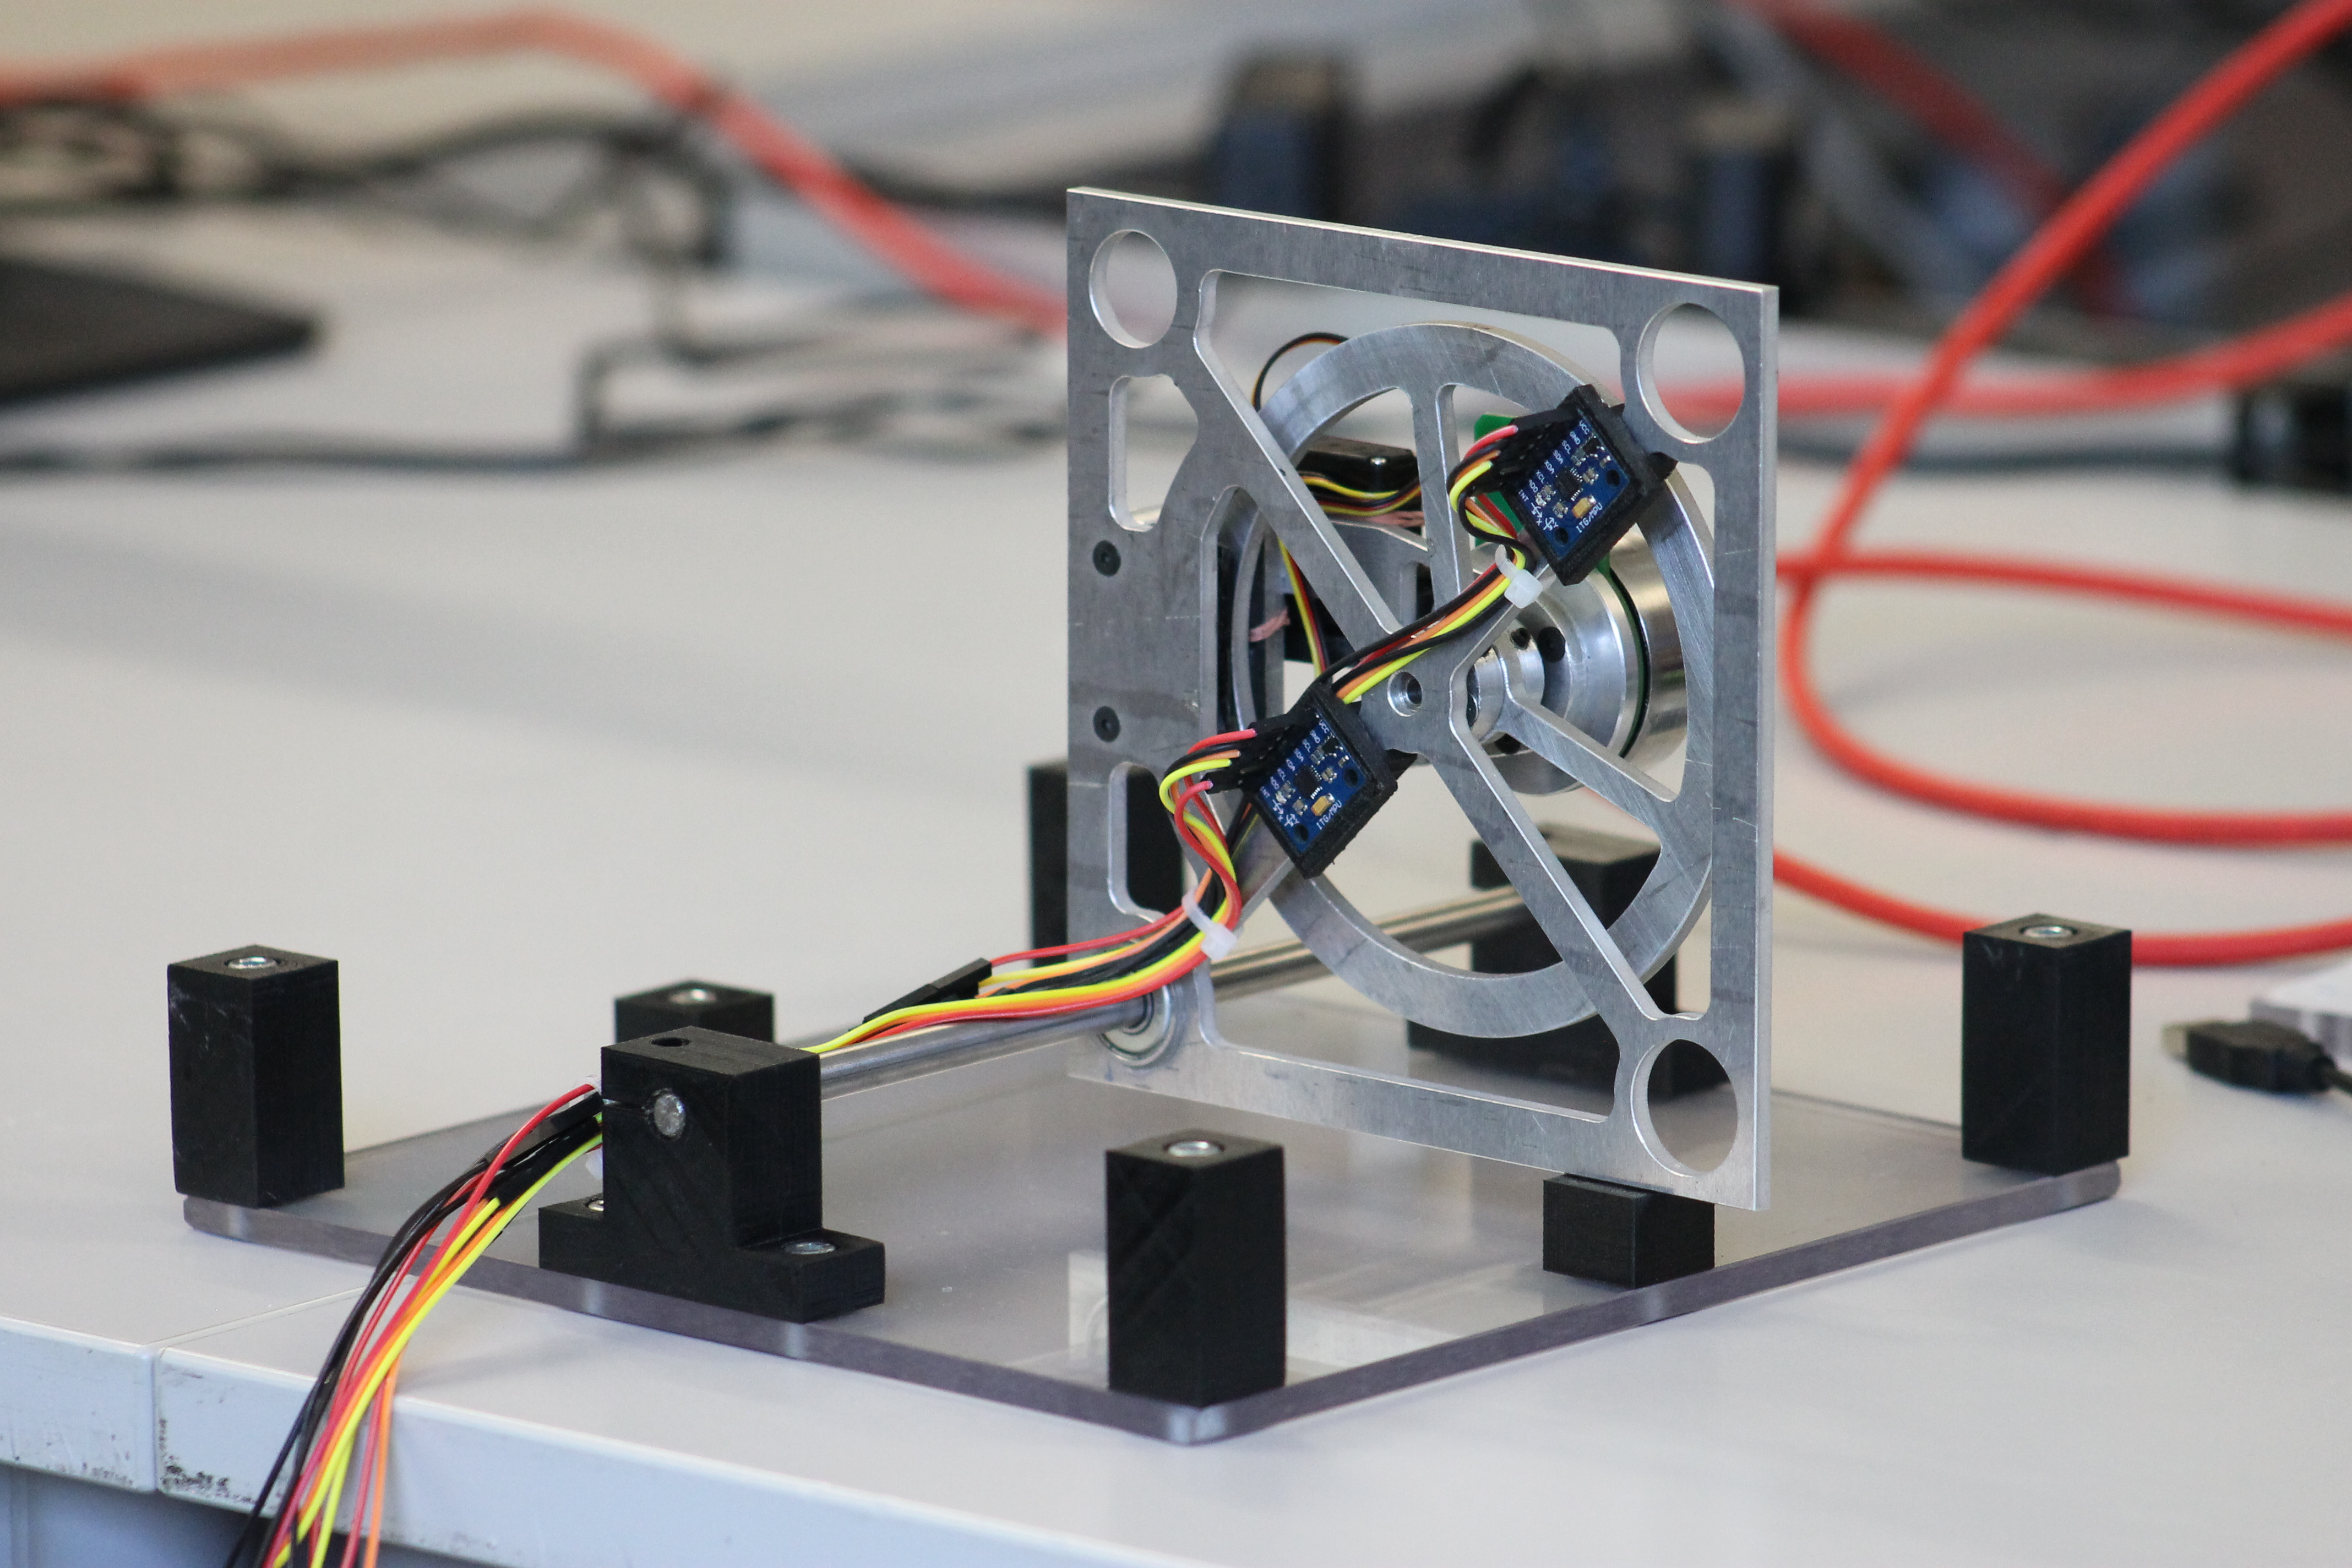
\includegraphics[width=\linewidth]{img/1D_Model_pic.JPG}
\caption{1D-Modell, Quelle: eigene Darstellung}
\end{figure}